% Figure S5: learning curves. Rendered by render_tables.py via render_figures.learning_curves from the sealed
% report-ready tables of the training diagnostics; nothing numeric is typed here.
\begin{figure}[!htbp]
\centering
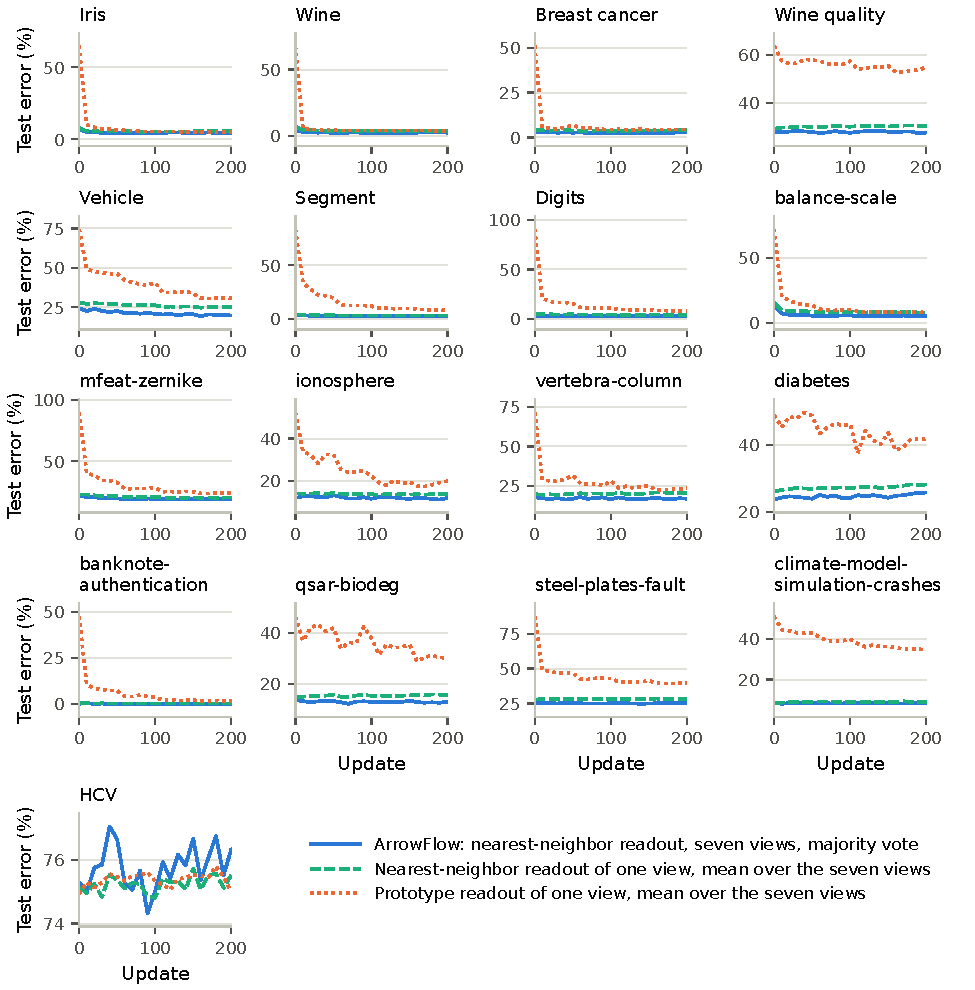
\includegraphics[width=\textwidth]{figures/data/figS_learning_curves.pdf}
\caption{\textbf{Training diagnostics: learning curves.} Test error in percent on the outer test rows against the number of updates, every ten updates from the initial filters, update 0, to update 200, for one fitting seed; each point is the mean over the 15 outer folds. Solid: ArrowFlow's seven-view nearest-neighbor readout, combined by majority vote. Dashed: the nearest-neighbor readout of one view, and dotted: the prototype readout of one view, each averaged over the seven views. The curves follow the filters through training, while the network that ArrowFlow returns is the one at its checkpoint (Table~\ref{tab:s-diag-checkpoints}). Each panel has its own error scale. Descriptive: nothing is selected or tested. At update 200 the prototype readout of one view has higher test error than the nearest-neighbor readout of one view on 15 of the 17 datasets. HCV: hepatitis C virus.}
\label{fig:learning-curves}
\end{figure}
